\documentclass[preprint, 12pt]{elsarticle}
\usepackage{amssymb,amsmath,amsthm}
\usepackage{graphicx}
\usepackage{url}
\usepackage{subfigure}

\newtheorem{thm}{Theorem}
\newtheorem{lem}{Lemma}
\newtheorem{conj}{Conjecture}
%\newproof{proof}{Proof}

\DeclareMathOperator{\od}{d}
\DeclareMathOperator{\vol}{v}
\DeclareMathOperator{\cog}{c}
\DeclareMathOperator{\svol}{\bar{\vol}}
\newcommand{\drop}{\downarrow}
\newcommand{\R}{\mathbb{R}}
\newcommand{\ud}{\mathrm{d}}

\newcommand{\eqlabel}[1]{\label{eq:#1}}
\renewcommand{\eqref}[1]{(\ref{eq:#1})}



\begin{document}
\begin{frontmatter}

\title{Oja Centers and Centers of Gravity\tnoteref{t1}}
\tnotetext[t1]{This work was initiated during the Workshop on Computational Geometry 2006 in Caldes de Malavella. The authors wish to thank Ferran Hurtado and the organizers for the opportunity of working on this topic.}

\author{Dan Chen}
\ead{dchen4@connect.carleton.ca}
\address{School of Computer Science, Carleton University}

\author{Olivier Devillers}
\ead{Olivier.Devillers@sophia.inria.fr}
\address{INRIA Sophia Antipolis — M\'editerran\'ee, France.}

\author{John Iacono}
\ead{jiacono@poly.edu}
\address{Department of Computer and Information Science, Polytechnic University}

\author{Stefan Langerman}
\ead{stefan.langerman@ulb.ac.be}
\address{D\'epartement d'Informatique, Universit\'e Libre de Bruxelles}

\author{ Pat Morin}
\ead{morin@scs.carleton.ca}
\address{School of Computer Science, Carleton University}


\begin{abstract}
\emph{Oja depth} (Oja 1983) is a generalization of the median to
multivariate data that measures the centrality of a point $x$ with respect
to a set $S$ of points in such a way that points with smaller Oja depth
are more central with respect to $S$.  Two relationships involving
Oja depth and centers of mass are presented.  The first is a form of
Centerpoint Theorem which shows that the center of mass of the convex
hull of a point set has low Oja depth.  The second is an approximation
result which shows that the center of mass of a point set approximates
a point of minimum Oja depth.
\end{abstract}


\end{frontmatter}

\section{Introduction}

Given a set $S$ of $n$ points in $\mathbb{R}^{d}$, the \emph{Oja depth}
\cite{Oja83} of a point $x\in\R^d$ is
\[ 
   \od(x, S) 
      = \sum_{y_{1},\ldots , y_{d} \in \binom{S}{d}} 
         \vol(x, y_{1}, \ldots, y_{d}) \enspace ,
\]
where $\vol(p_{1},\ldots, p_{d+1})$ denotes the volume of the simplex
whose vertices are $p_{1}\ldots p_{d+1}$.\footnote{In Oja's original
definition, the sum is normalized by dividing by $\binom{|S|}{d}$. We omit this here since it changes none of our results and clutters our formulas.}
A point in $\mathbb{R}^{d}$ with the minimum Oja depth is called an
\emph{Oja center}.

\subsection{New Results}

In this paper we consider relationships between centers of mass of
certain sets and Oja depth. The \emph{center of mass} of a finite
point set $S\subset\R^d$ is the average of those points,
\[
  \cog(S) = |S|^{-1}\sum_{x\in S} x \enspace .
\]
If $P\subset\R^d$ is a bounded object of non-zero volume, the center of mass of $P$ is
\[
  \cog(P) = \frac{\int_{x \in P} x\, \ud x}{\vol(P)} \enspace .
\]

In this paper, we prove the following results about the Oja depth of an
$n$ point set $S$, whose convex hull $A$ has unit volume and that has an Oja center $x$:

\begin{equation}
  \od(\cog(A),S) \le \binom{n}{d}/(d+1) \enspace ,
   \eqlabel{centerpoint}
\end{equation}
\begin{equation}
  \od(\cog(S),S) \le (d+1)\od(x,S) \enspace .
   \eqlabel{approx}
\end{equation}

The bound in \eqref{centerpoint} is not known to be tight. The bound
in \eqref{approx} is tight, up to a lower-order term, for some point
sets $S$.

\subsection{Related Results}

Our first result, \eqref{centerpoint}, is a form of \emph{Centerpoint
Theorem} that upper-bounds the Oja depth of $\cog(A)$, and hence
also the Oja depth of $x$, in terms of the volume of the convex hull
of $S$.  Previously, centerpoint theorems were known for other depth
functions such as Tukey depth~\cite{m02,pa95,t71} and simplicial depth~\cite{b82,bf84,l90}.  To the best of our knowledge, this is the first
such result for Oja depth.

Our next result, \eqref{approx}, can be viewed in two
ways: 
\begin{enumerate}
  \item The first is a linear-time algorithm to find a point whose depth is a constant factor approximation
  of the depth of the Oja center.  In 1-d, Oja depth is minimized by the
  median, which can be found in $O(n)$ time. However, in 2-d, the best
  known algorithm for minimizing Oja depth exactly takes $O(n\log^3 n)$
  time~\cite{alst03}.  Approximation algorithms for minimizing Oja depth,
  based on uniform grids and sampling from $\binom{S}{d}$, are given by
  Ronkainen, Oja, and Orponen~\cite{roo01}; this algorithm and several others are implemented in the R-package, OjaNP~\cite{ojanp}.  However, in pathological
  cases, their approximation algorithm is not guaranteed (or even likely)
  to find a point that closely approximates the Oja center, either in
  terms of distance or in terms of its Oja depth.\footnote{This follows
  from the fact that the value of the Oja depth function and the location
  of the Oja center can be arbitrarily different for two sets $S_1$
  and $S_2$ that differ in only $d$ points~\cite{not90}.}

  \item Another view of \eqref{approx} is that it gives insight into
  the Oja depth function and the Oja center.  In some sense, it tells
  us that the Oja center is not terribly different from the center of
  mass of $S$, since the center of mass of $S$ minimizes, to within a
  constant factor, the Oja depth function.
\end{enumerate}

\section{Oja Center and Mass Center of $\mathbf{A}$}
%\label{sec:cnterofA}
\label{sec:gravcenter}

In this section, we relate the Oja depth of the center of mass of the
convex hull of $S$ to the volume of the convex hull of $S$.  Throughout
this section, $A$ denotes the convex hull of $S$ and we assume, without
loss of generality, that $\vol(A)=1$.

Our upper-bound is based on the following \emph{central identity}:
For any disjoint sets $X,Y\subseteq\R^d$ with $\vol(X\cup Y) > 0$,
\[
   \cog(X \cup Y) = \frac{\vol(X)\cog(X) + \vol(Y)\cog(Y)}{\vol(X \cup Y)}.
\]
We first give an inductive proof of our result for point sets in $\R^2$,
and then give a proof for point sets in $\R^d$ that uses tools from
convex geometry.

\subsection{An Upper Bound in $\mathbb{R}^{2}$}
\label{sec:2dbound}

The following result shows that, for a convex polygon $E$ (e.g., $E=A$),
it is not possible to form an overly-large triangle that has $\cog(E)$
as one of its vertices:

\begin{lem}
  \label{lem:2dgrav}
  Let $A$ be a convex polygon and let $p_{1}$ and $p_{2}$ be any two points in $A$. Then $\vol(p_{1},p_{2},\cog(A)) \leq \vol(A)/3$.
\end{lem}
\begin{proof}
Assume, without loss of generality, that $p_1p_2$ is horizontal and that
$\cog(A)$ is above $p_1p_2$.  We may assume that $p_1p_2$ is edge of $A$
since, otherwise, we can remove the part of $A$ that is below $p_1p_2$.
This decreases $\vol(A)$ and moves $\cog(A)$ further away from the segment $p_1p_2$, which increases $\vol(\cog(A),p_1,p_2)$.

The proof is by induction on the number of vertices of $A$.  If $A$
is a triangle then one can easily verify the result.  Therefore,
assume $A$ has $n\ge 4$ vertices.  Consider an edge $ab$ of $A$ where
$a\neq p_2$ is adjacent to $p_1$ and let $c\neq a$ be adjacent to $b$
(see Figure~\ref{fig:inductive}).  Since $A$ has 4 or more vertices,
we may assume that the $y$-coordinate of $b$ is not smaller than the
$y$-coordinate of $a$. Otherwise we can reverse the roles of $p_1$
and $p_2$ and redefine $a$ and $b$ with respect to the new $p_1$.

Draw a ray $r$ whose origin is at $p_1$ and such that the triangle $t_1$
supported by $p_1a$, $ab$ and $r$ and the triangle $t_2$ supported by
$r$, $ab$, and the line through $bc$ have the same area.  Such a ray is
guaranteed to exist by a standard continuity argument that starts with
$r$ containing $a$ and rotates about $p_1$ until $r$ contains $b$.

\begin{figure*}[htbp]
  \begin{center}
    \begin{tabular}{cc}
      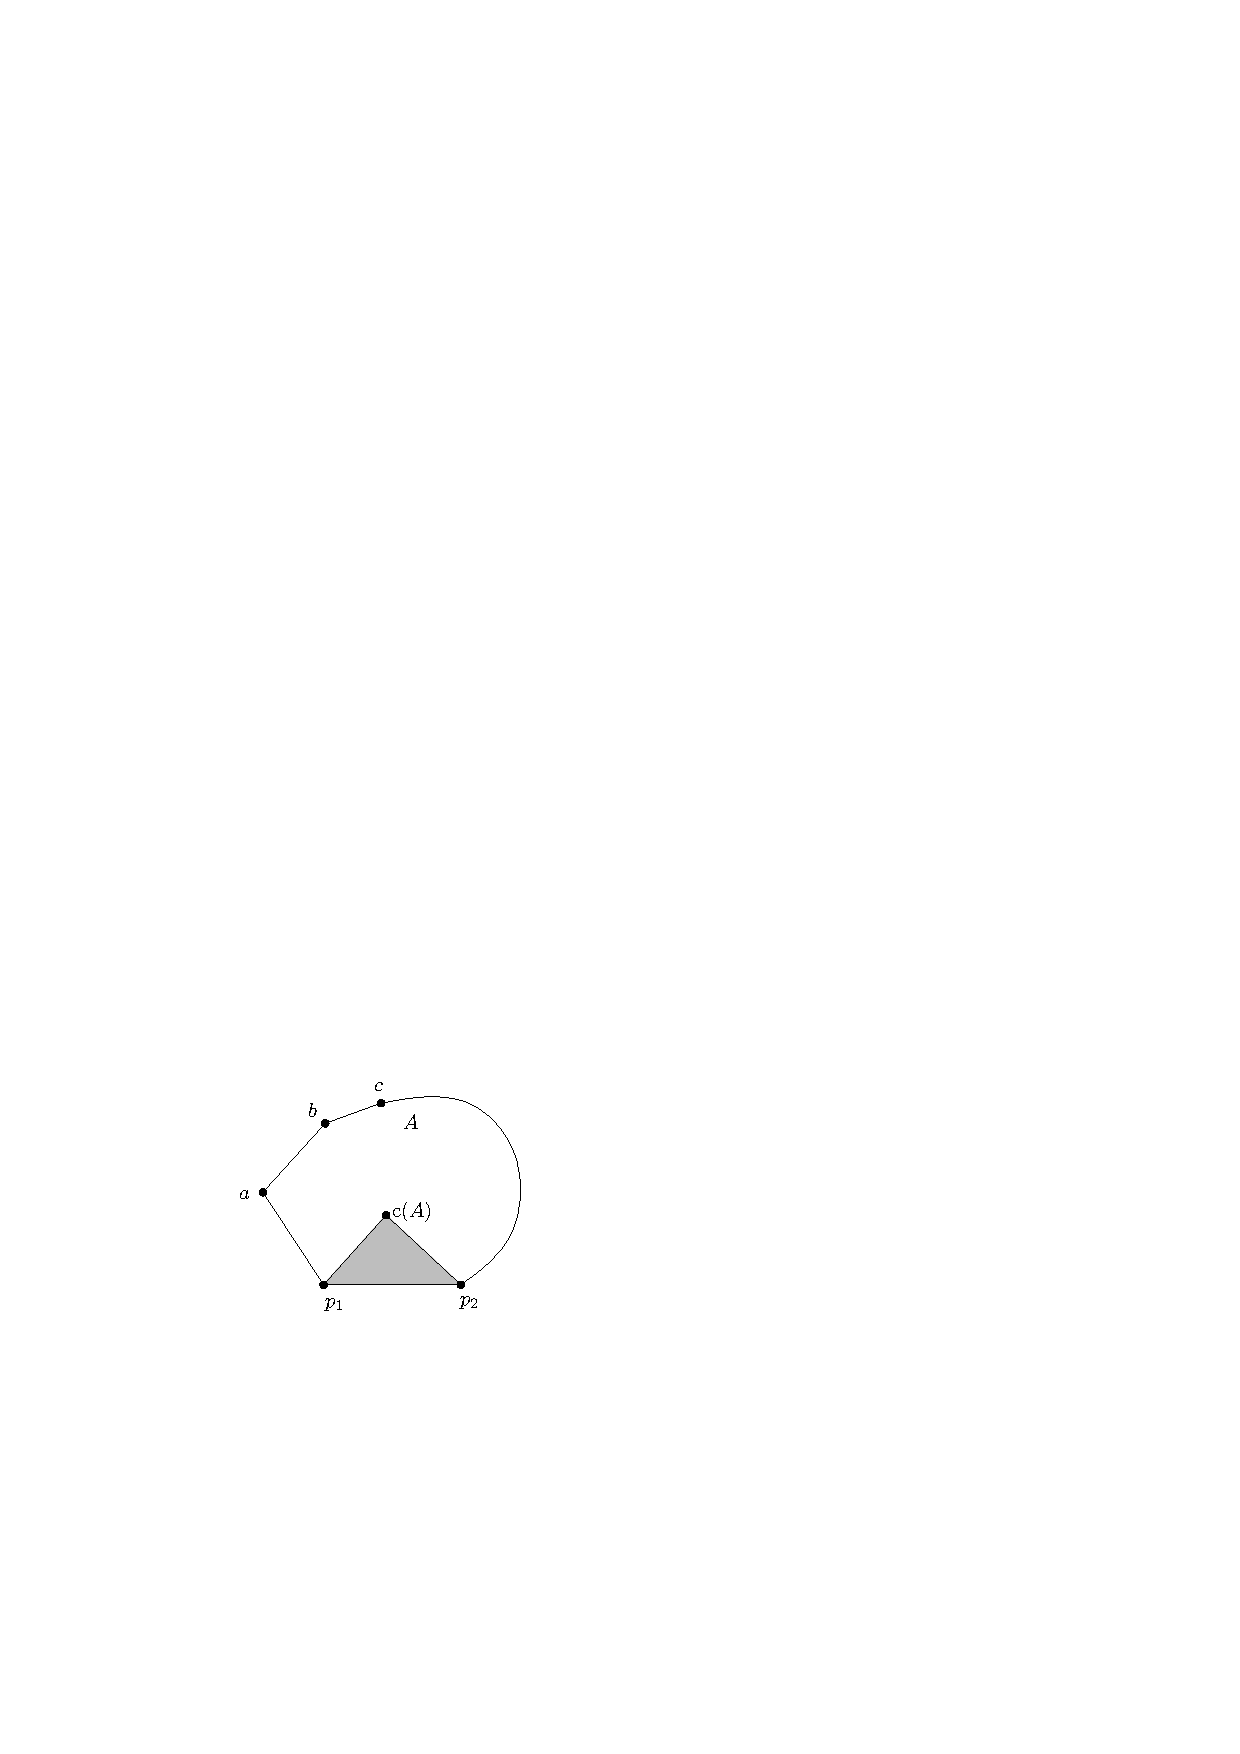
\includegraphics{pics/inductive} &
      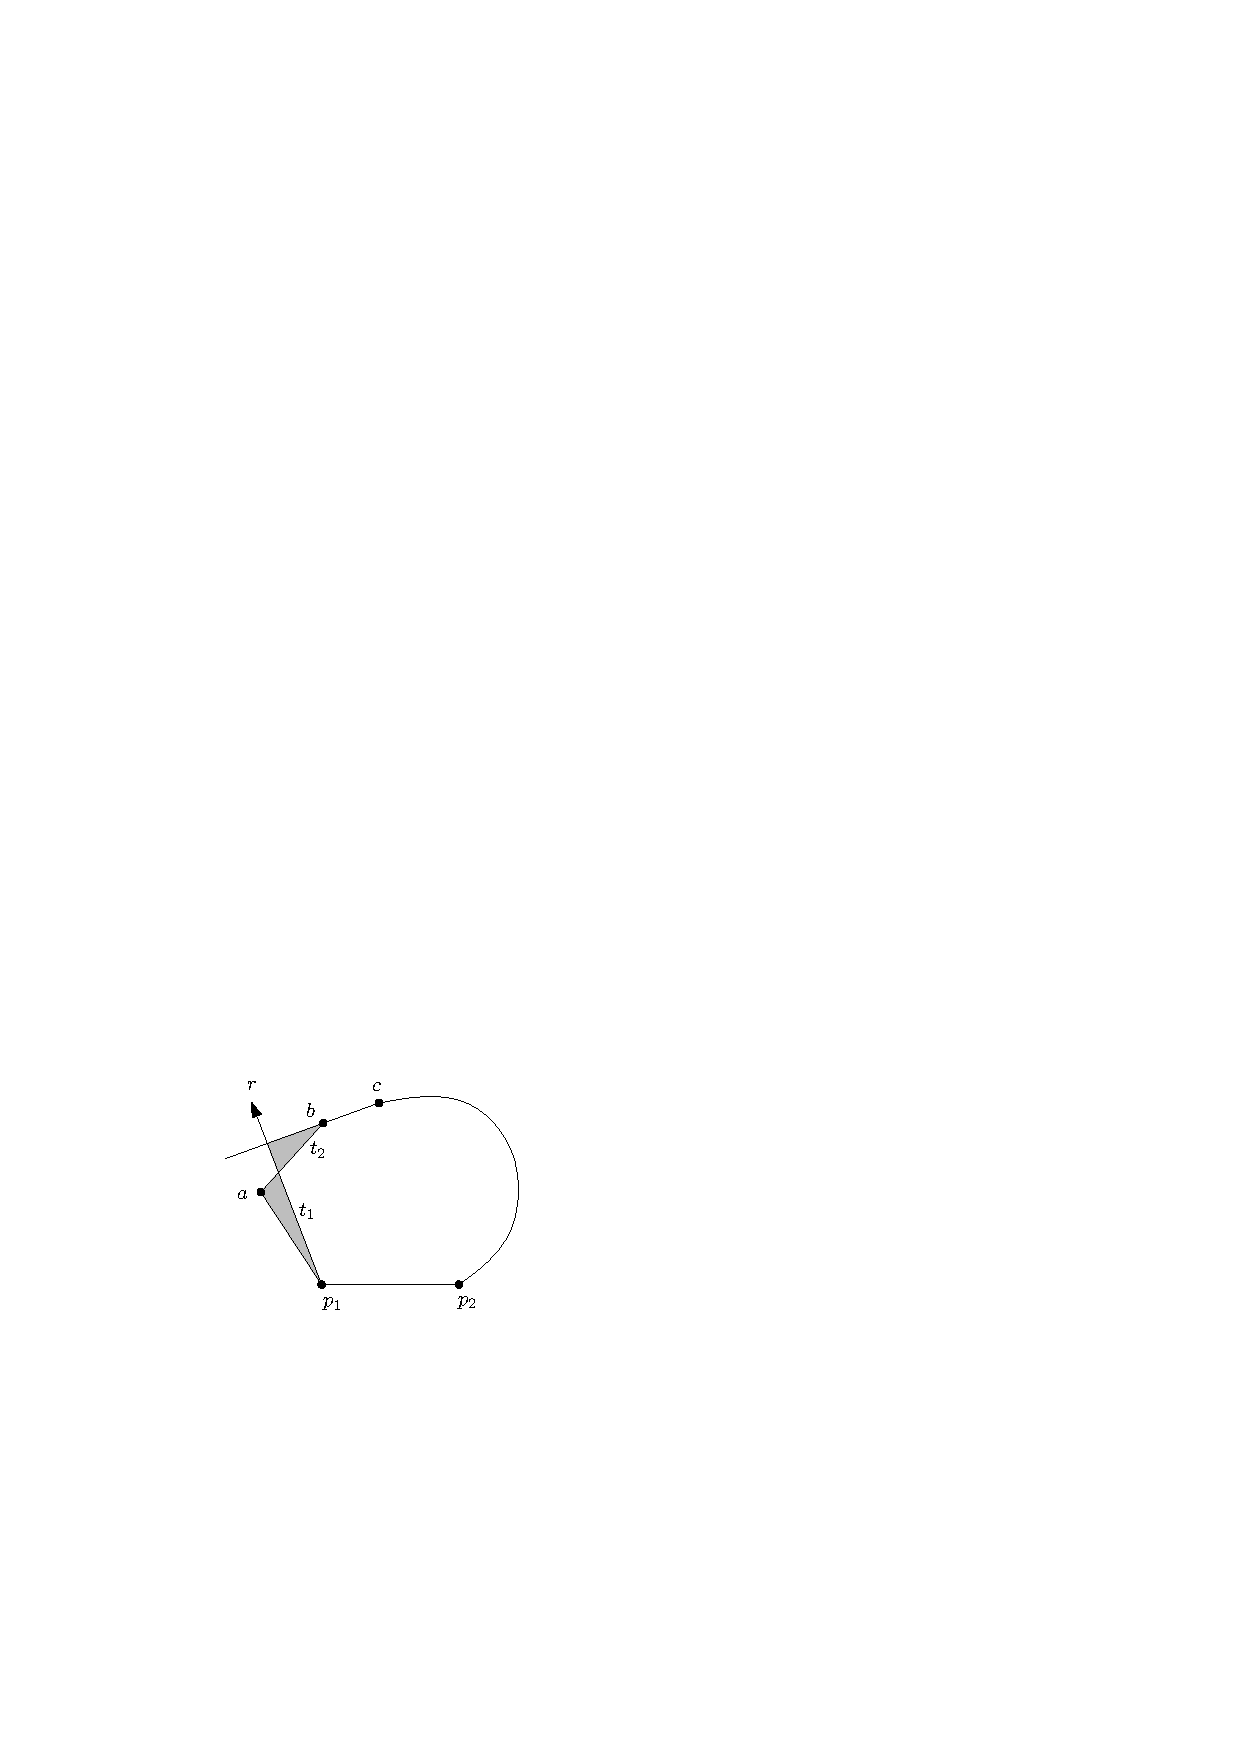
\includegraphics{pics/inductive2} \\
      \multicolumn{2}{c}{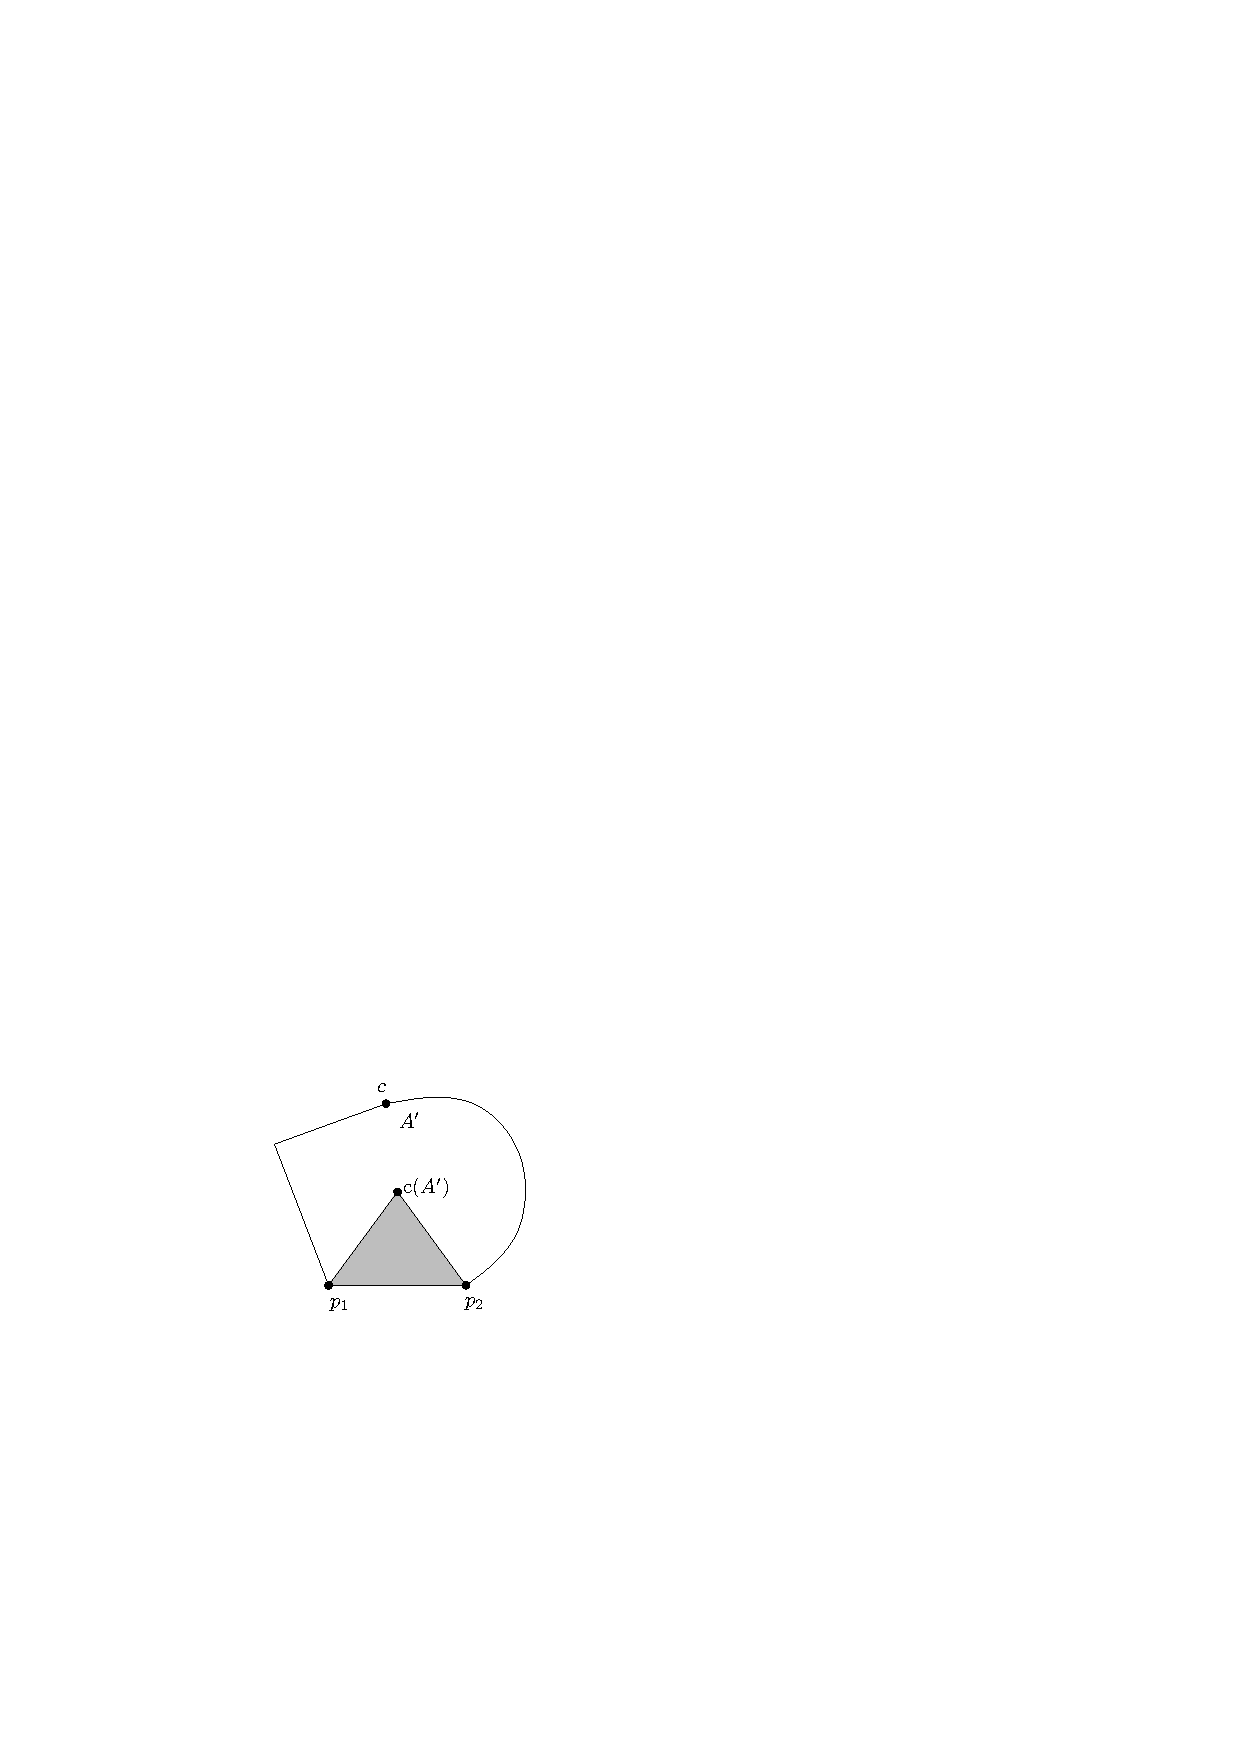
\includegraphics{pics/inductive3}}
    \end{tabular}
  \end{center}
  \caption{The proof of Lemma~\ref{lem:2dgrav}.}
  \label{fig:inductive}
\end{figure*}

Now, convert $A$ into a polygon $A'$ by removing $t_1$ and adding $t_2$.
This does not change the area of $A$.  Furthermore, since $t_1$ and
$t_2$ are separated by a horizontal line, with $t_2$ above $t_1$, this
implies that the $\cog(A')$ has a larger $y$-coordinate than $\cog(A)$,
so $\vol(\cog(A),p_1,p_2)) \le \vol(\cog(A'),p_1,p_2)$.  Note, also, that $A'$
has $n-1$ vertices so, by induction,
\[
  \vol(\cog(A),p_1,p_2) \le \vol(\cog(A'),p_1,p_2) \le \vol(A')/3 = \vol(A)/3 \enspace ,
\]
completing the proof.
\end{proof}

\begin{thm}
  \label{thm:2dcenter}
  Let $S$ be a set of points in $\R^2$ whose convex hull, $A$, has unit area. Then $\od(\cog(A),S)\le n^2/6$.
\end{thm}

\begin{proof}
  Applying Lemma~\ref{lem:2dgrav}, we immediately get
\[\od(\cog(A), S) = \sum_{p_{1},p_{2}\in \binom{S}{2}} \vol(p_{1},p_{2},\cog(A)) \leq \binom{n}{2}/3 < \frac{n^{2}}{6}\enspace ,\]
as required.
\end{proof}


\subsection{An Upper Bound  in  $\mathbb{R}^{d}$}

In this section, we extend our bound to $\R^d$. However, it seems
difficult to apply induction to polytopes in $\R^d$, so we resort to
some tools from convex geometry.

Let $A$ be a convex body in $\mathbb{R}^{d}$, where $d \geq 2$. Suppose
$A$ lies between parallel hyperplanes $x_{1} = a$ and $x_{1} = b$,
where $a < b$. For each $x$ with $a \leq x \leq b$, let $A_{x}$ be the
intersection of $A$ with the hyperplane $x_{1} = x$, and define $r_{x}$
by the equation
\[ \omega_{d-1}r_{x}^{d-1} = \vol_{d-1}(A_{x})\enspace , \]
where $\vol_{d-1}(X)$ denotes the $(d-1)$-dimensional volume of $X$ and
$\omega_{d-1}$ is the $(d-1)$-dimensional volume of the unit $(d-1)$-ball.
In this way, $r_{x}$ is the radius of a $(d-1)$-ball whose $(d-1)$-dimensional volume is the same as that of $A_{x}$. For each $a \leq x \leq b$, let $C_{x}$ be defined by the equation
\[ C_{x} = \{ (x, x_{2}, \ldots, x_{d}) : x_{2}^{2} + \cdots + x_{d}^{2} \leq r_{x}^{2} \}. \]
Then the set
\[ C = \cup \{C_{x} : a \leq x \leq b\} \]
is called the \emph{Schwarz rotation-symmetral} of $A$ in the $x_{1}$-axis.
For example, in $\R^3$, $C$ is a stack of disks perpendicular to, and
centered on, the $x$-axis. Each disk has the same area as the corresponding
slice of $A$.

\begin{thm}[Webster~\cite{Webs95}]
  \label{thm:webs}
  Let $A$ be a convex body in $\mathbb{R}^{d}$ $(d \geq 2)$ whose Schwarz rotation-symmetral in the $x_{1}$-axis is $C$. Then $C$ is a convex body having the same volume as $A$.
\end{thm}


\begin{lem}
  \label{lem:simpvol}
  Let $P$ be a convex polytope in $\R^d$ and let $p_1,\ldots,p_d$ be any $d$ points in $P$.  Then $\vol(p_1,\ldots,p_d,\cog(P))\le \vol(P)/(d+1)$.
\end{lem}

\begin{proof}

  Our proof of this lemma is based on the fact that the center of mass of a cone or pyramid with height $\ell$ in $\mathbb{R}^{d}$ has distance $\frac{\ell}{d+1}$ from the base. To see this, we assume that base of the cone of pyramid contains the origin and is perpendicular to the $x_{1}$-axis. According to central identity, the $x_1$-value of the center of mass is
\[
\frac{\int_{0}^{\ell} x_1 a (\ell - x_1)^{d-1} \ud x_1 }{\frac{a \ell^{d-1} \ell}{d}},
\]
where $a$ is the constant involved in the computing the $(d-1)$-dimensional volume of the base. Solving this integration we get $\frac{\ell}{d+1}$~\cite{edwards98}.

Let $h$ be a hyperplane that contains $p_1,\ldots,p_d$.  If $\cog(P)$ is
in $h$, or $p_1,\ldots,p_d$ are not in general position, $\vol(p_1,\ldots,p_d,\cog(P)) = 0$ and there is nothing to
prove. Otherwise, rotate $P$ to make $h$ perpendicular to the $x_{1}$-axis
with $\cog(P)$ above $h$. If there is any volume of $P$ below $h$, we can
cut that part off from $P$ to obtain a new polytope $P'$.  The volume
of $P'$ will be less than that of $P$, and its center of mass $\cog(P')$ will
be above $\cog(P)$.  In this way, if $(P,p_1,\ldots,p_d)$ is a counterexample
to the lemma, then so is $(P',p_1,\ldots,p_d)$. 

The face, $B$, of $P'$ in $h$ contains $p_1,\ldots,p_d$. If $P'$ is a pyramid, we have 
\[
\vol(p_1,\ldots,p_d,\cog(P'))
   \le \vol(B,\cog(P')) 
   = \vol(P')/(d+1) \le \vol(P)/(d+1)\enspace .
\]
If $P'$ is not a pyramid, let $q$ be a
point on the $x_1$ axis, above $h$, and such that the pyramid $D$ with
$B$ as base and $q$ as apex has the same volume as $P'$.  Let $C$ be the
Schwarz rotation-symmetral of $P'$ in the $x_{1}$-axis, and $R$ be that
of $D$ (see Figure~\ref{fig:rotsym}). Note that $R$ is a conic pyramid.
By Theorem~\ref{thm:webs}, $C$ is convex and $\vol(C) = \vol(P') =
\vol(R)$. Let $c$ be the intersection of the surfaces of $C$ and $R$
above $B$. Note that the surface of $R$ is bounded by a collection of
lines that pass through $q$.  By convexity, each of these lines intersects $C$ in at
most 2 points.  One of these points has the same $x_1$-coordinate as $B$
and the other points lie on the boundary of a $(d-1)$-ball $c$.
\begin{figure}[ht]
  \centering
  \subfigure[]{\label{fig:pol}
    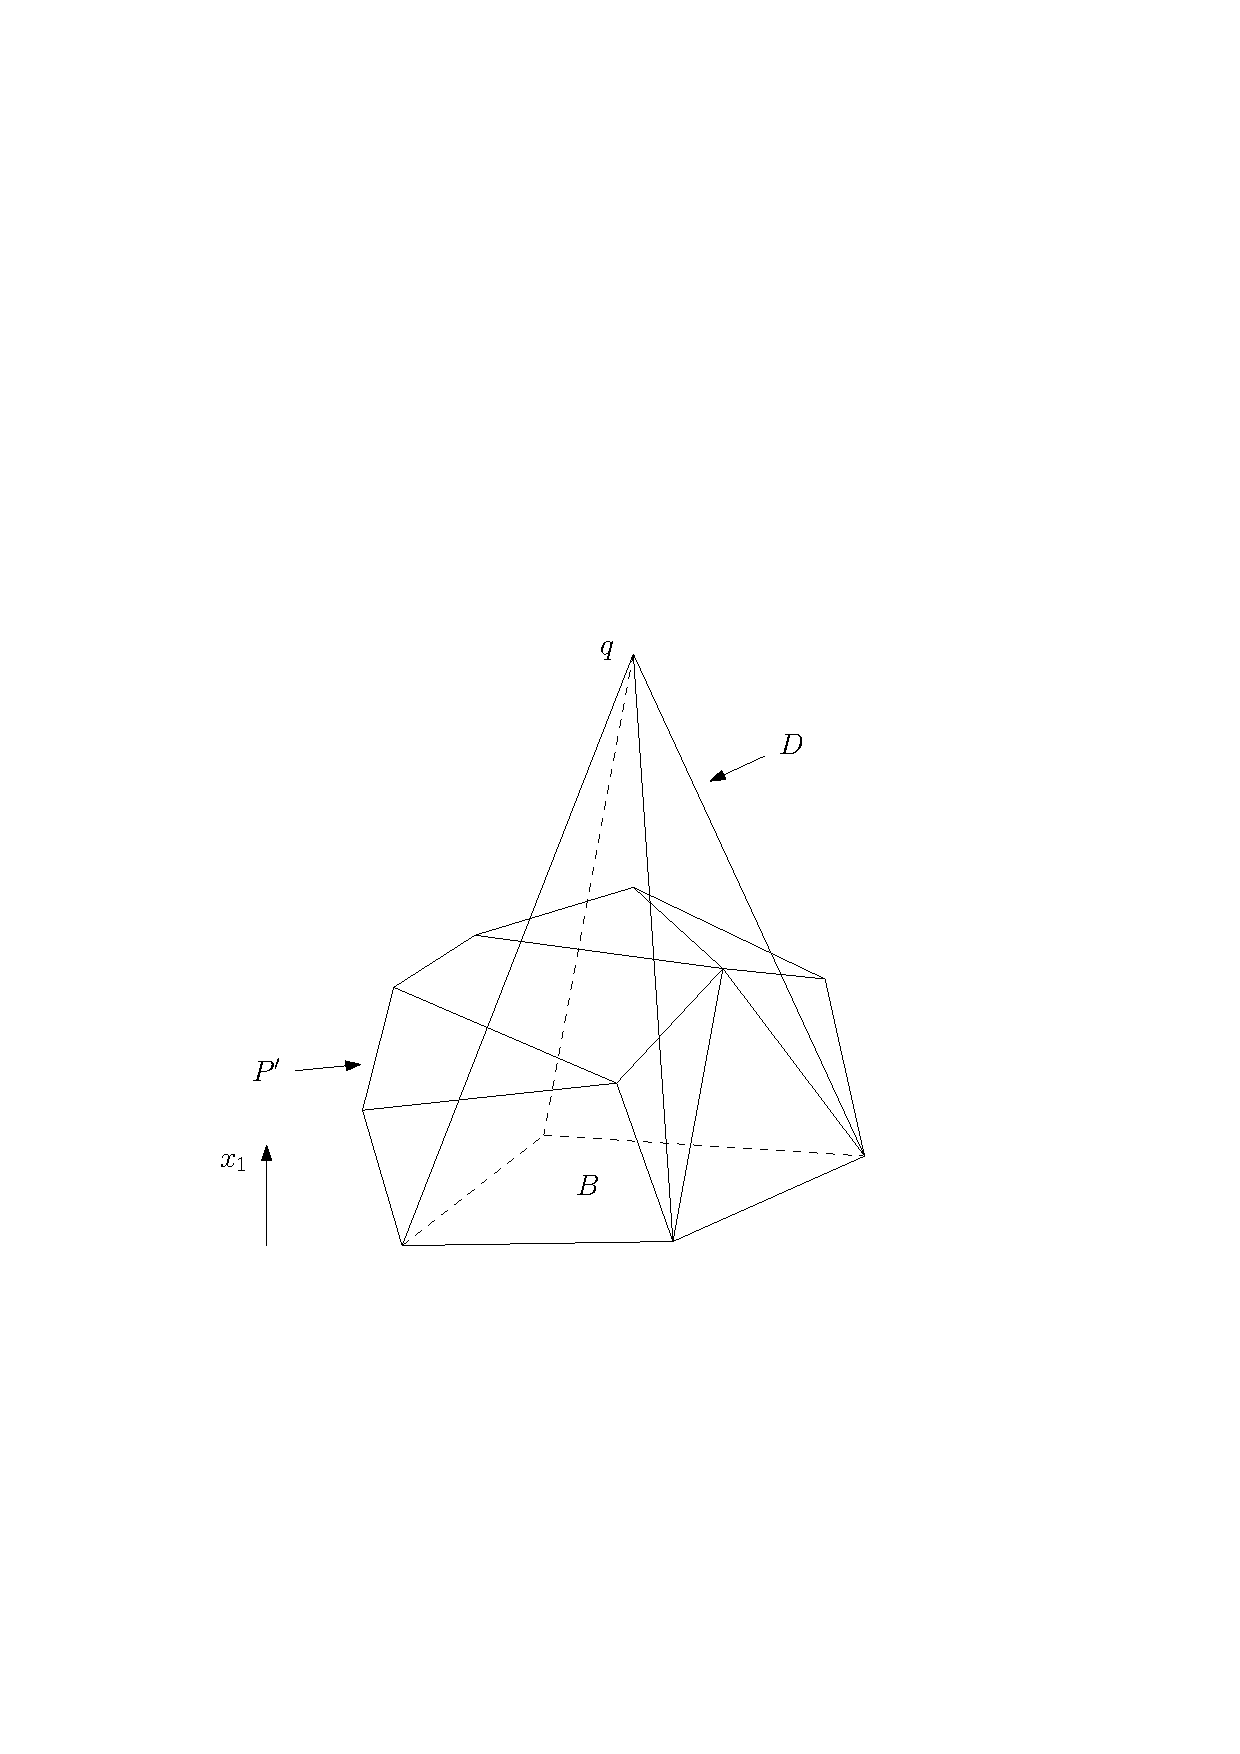
\includegraphics[width=0.42\textwidth]{pics/polpyr.pdf}
  }
  \hspace{5mm}
  \subfigure[]{\label{fig:rot}
    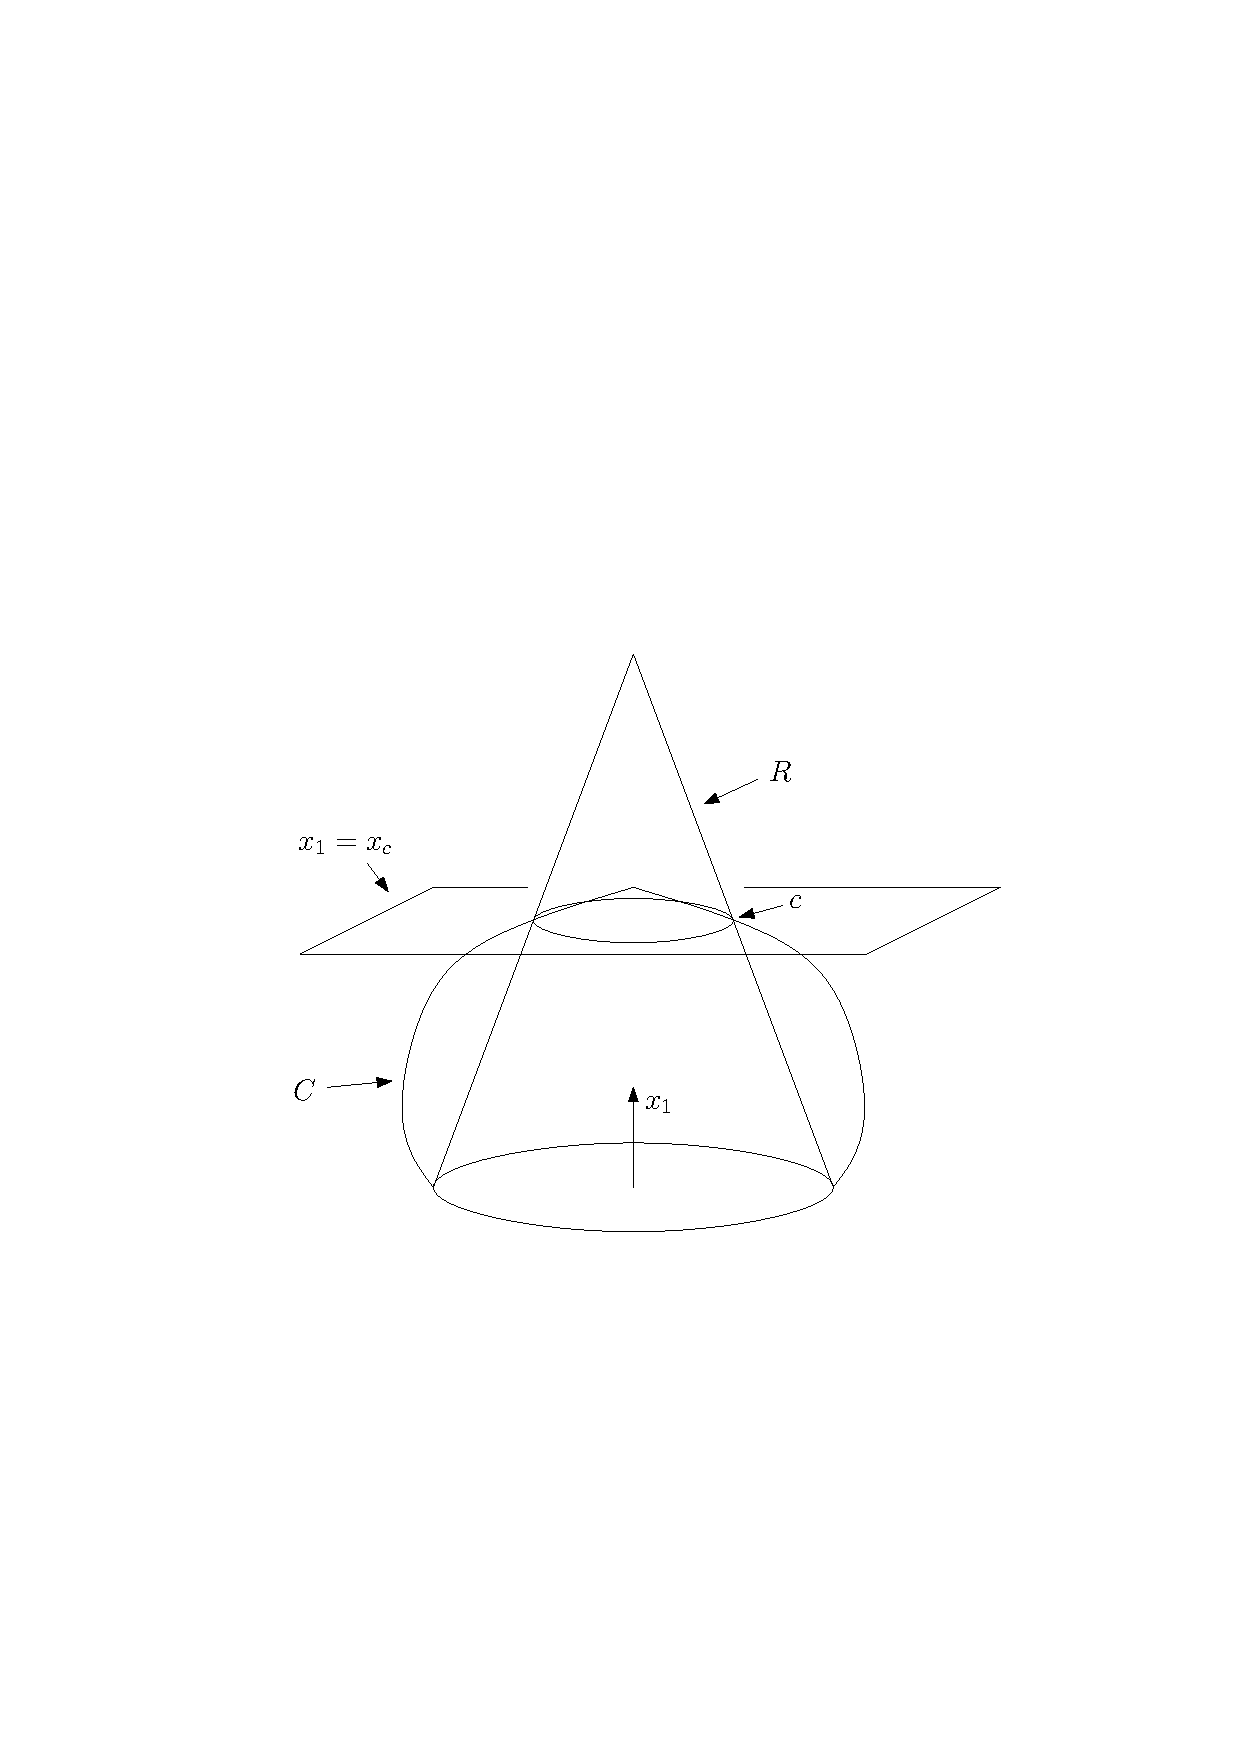
\includegraphics[width=0.48\textwidth]{pics/rotsym.pdf}
  }
  \caption{The Schwarz rotation-symmetral of $P'$ and $D$}
  \label{fig:rotsym}
\end{figure}

%By
%the definition of Schwarz rotation-symmetral, the volume of $C$ that is
%outside of $R$ is below $x_{c}$, and the volume of $R$ outside of $C$
%is above $x_{c}$. According to central identity, we have
Let $x_{c}$ be the $x_{1}$-coordinate of $c$. Since $C$ is convex and
 a rotation symmetral, $C\setminus R$ is below the hyperplane $x_{1}
 = x_{c}$.  Furthermore, $R\setminus C$ is above the hyperplane
 $x_1=x_{c}$. By the central identity, we have
\[
\cog(R) = \frac{\vol(R \cap C)\cog(R \cap C) + \vol(R \setminus C)\cog(R \setminus C)}{\vol(R)},
\]
and
\[
\cog(C) = \frac{\vol(R \cap C)\cog(R \cap C) + \vol(C \setminus R)\cog(C \setminus R)}{\vol(C)}.
\]
Since $\cog(R \setminus C)$ is above $\cog(C \setminus R)$, $\cog(R)$ is above $\cog(C)$.

The centers of mass of $P'$ and $C$ have the same $x_1$ value because, in the
Schwarz rotation-symmetral, $C_{x}$ has the same $x_{1}$ value as $A_{x}$.
So do the centers of mass of $D$ and $R$. Since $D$ is a pyramid, the convex hull of $p_1,\ldots,p_d$ is contained
in $B$,  $\cog(P)$ is below $\cog(P')$, and $\cog(P')$ is below $\cog(D)$, we have 
\[ \vol(p_1,\ldots,p_d,\cog(P')) \leq \vol(P')/(d+1) \leq \vol(P)/(d+1).\]
To see why the first inequality is true, observe that 
\[
  \begin{aligned}
    \vol(p_1,\ldots,p_d,\cog(P')) &
   \le \vol(B,\cog(P')) 
   = \vol(B,\cog(C)) \\
   & \le\vol(B,\cog(D))= \vol(R)/(d+1) = \vol(P')/(d+1) \enspace .
  \end{aligned}
\]
This completes the proof.
\end{proof}

The bound in Lemma~\ref{lem:simpvol} is tight, for example, when $S$
consists of the $d+1$ vertices of a simplex. Next we show how this
relates to Oja depth:

\begin{thm}
  \label{thm:ndcenter}
  Let $S$ be a set of points in $\R^d$ whose convex hull, $A$, has unit volume. Then $\od(\cog(A),S)\le \binom{n}{d}/(d+1)$.
\end{thm}

\begin{proof}
  \[
    \begin{aligned}
     \od(\cog(A), S) 
      & = \sum_{y_{1},\ldots , y_{d} \in \binom{S}{d}} \vol(\cog(A), y_{1}, \ldots,
y_{d}) \\
      & \leq \binom{n}{d}/(d+1) \enspace ,
    \end{aligned} \]
where the inequality is an application of Lemma~\ref{lem:simpvol}.
\end{proof}
% Does any other point has smaller upper bound?

\section{Oja Center and Mass Center of $\mathbf{S}$}
\label{sec:cnterofS}

In this section, we show that the center of mass of $S$ provides
a constant-factor approximation to the point of minimum Oja depth.
We begin by proving the result for point sets in 1 dimension:

\begin{lem}
\label{lem:grav1d}
For any finite set $S\subset\mathbb{R}$, and any $x\in\mathbb{\R}$, $\od(\cog(S),S) \le 2\od(x,S)$.
\end{lem}

\begin{proof}
Denote the elements of $S$ by $p_1,\ldots,p_n$ in any order.  Let the
multiset $S_i$ contain $p_1,\ldots,p_i$ as well as $n-i$ copies of
$x$. 
Let $c_i=\cog(S_i)$.
We will show, by induction on $i$, that $\od(c_i,S_i)\le
2\od(x,S_i)$ for all $i\in\{0,\ldots,n\}$.  This is sufficient,
since $S_n=S$.

For the base case $S_0$ consists of $n$ copies of $x$, so
$c_0=x$ and $\od(c_0,S_0)= 0 = 2\od(x,S_0)$.  Next,
we assume that $\od(c_i,S_i) \le 2\od(x,S_i)$ and prove that
$\od(c_{i+1},S_{i+1}) \le 2\od(x,S_{i+1})$.  Note that
\[
   \od(x,S_{i+1}) = \od(x,S_i) + |p_{i+1}-x| \enspace .
\]
Furthermore, 
\[
   c_{i+1} = c_i + (p_{i+1}-x)/n \enspace ,
\]
so
\begin{align*}
    &\od(c_{i+1}, S_{i+1}) \\
     & =  \od(c_i, S_{i}) 
        + \sum_{q\in S_i} (|c_{i+1} - q| - |c_i - q|) 
        + (|c_{i+1} - p_{i+1}| - |c_{i+1} - x|) \\
     & \le  \od(c_i, S_{i}) 
         + n|p_{i+1}-x|/n  
         + (|c_{i+1} - p_{i+1}| - |c_{i+1} - x|) \\
     & \le  \od(c_i, S_{i}) + 2|p_{i+1}-x|  \\
     & \le  2\od(x, S_{i}) 
             + 2|p_{i+1}-x|  \\
     &  =  2\od(x, S_{i+1}) \enspace ,
\end{align*}
as required.
\end{proof}

We remark that the above proof uses little more than triangle
inequality. In particular, the same proof shows that the center of
mass gives a 2-approximation for the Fermat-Weber center in any
dimension.\footnote{The Fermat-Weber center of a point set $S$ in $\R^d$
is the point $x$ that minimizes $\sum_{y\in S}\|x-y\|$.}  Unfortunately,
in higher dimensions, Oja depth does not enjoy this nice property.

\begin{thm}
\label{thm:gravdd}
For any finite set $S\subseteq\mathbb{R}^d$,
$\od(\cog(S),S) \le (d+1)\od(x,S)$ for any $x\in\mathbb{R}^d$.
\end{thm}

\begin{proof}
The case $d = 1$ is covered by Lemma~\ref{lem:grav1d}, so we assume $d \ge 2$. In this proof, we will make use of the fact that, for any $d$-simplex $T$
with vertex set $V_T$ and a point
$q\in\mathbb{R}^d$,
\begin{equation}
  \vol(T) \le \sum_{p_1,\ldots,p_d\in\binom{V_T}{d}} \vol(p_1,\ldots,p_d,q)\enspace , 
   \label{eq:cover}
\end{equation}
since $T$ is contained in the union of the simplices on the right hand side. Equality occurs if $q$ is inside $T$.

Define $S_i$ as in the proof of Lemma~\ref{lem:grav1d}. Let $S'$ be
$S_{i+1}$ with one occurrence of $p_{i+1}$ removed. The induction and
base case are the same as in Lemma~\ref{lem:grav1d}. First, we have
\begin{eqnarray}
\od(x,S_{i+1}) 
   & = & \od(x,S_i) \nonumber \\ 
   && {} + \sum_{Q\in\binom{S_i}{d-1}} \vol(x,p_{i+1},Q). \label{eq:o}
\end{eqnarray}
and
\begin{align}
   \od(c_{i+1},S_{i+1}) 
   &  = \od(c_i,S_{i}) \nonumber \\
   &    \quad + \sum_{P \in \binom{S_i}{d}} 
           (\vol(c_{i+1}, P)- \vol(c_i,P))
              \label{eq:i} \\
   &   \quad + \sum_{Q\in \binom{S'}{d-1}}
           (\vol(c_{i+1},p_{i+1},Q)- \vol(c_{i+1},x,Q)).
            \label{eq:ii} 
\end{align}
\begin{figure}[htb]
  \begin{center}
    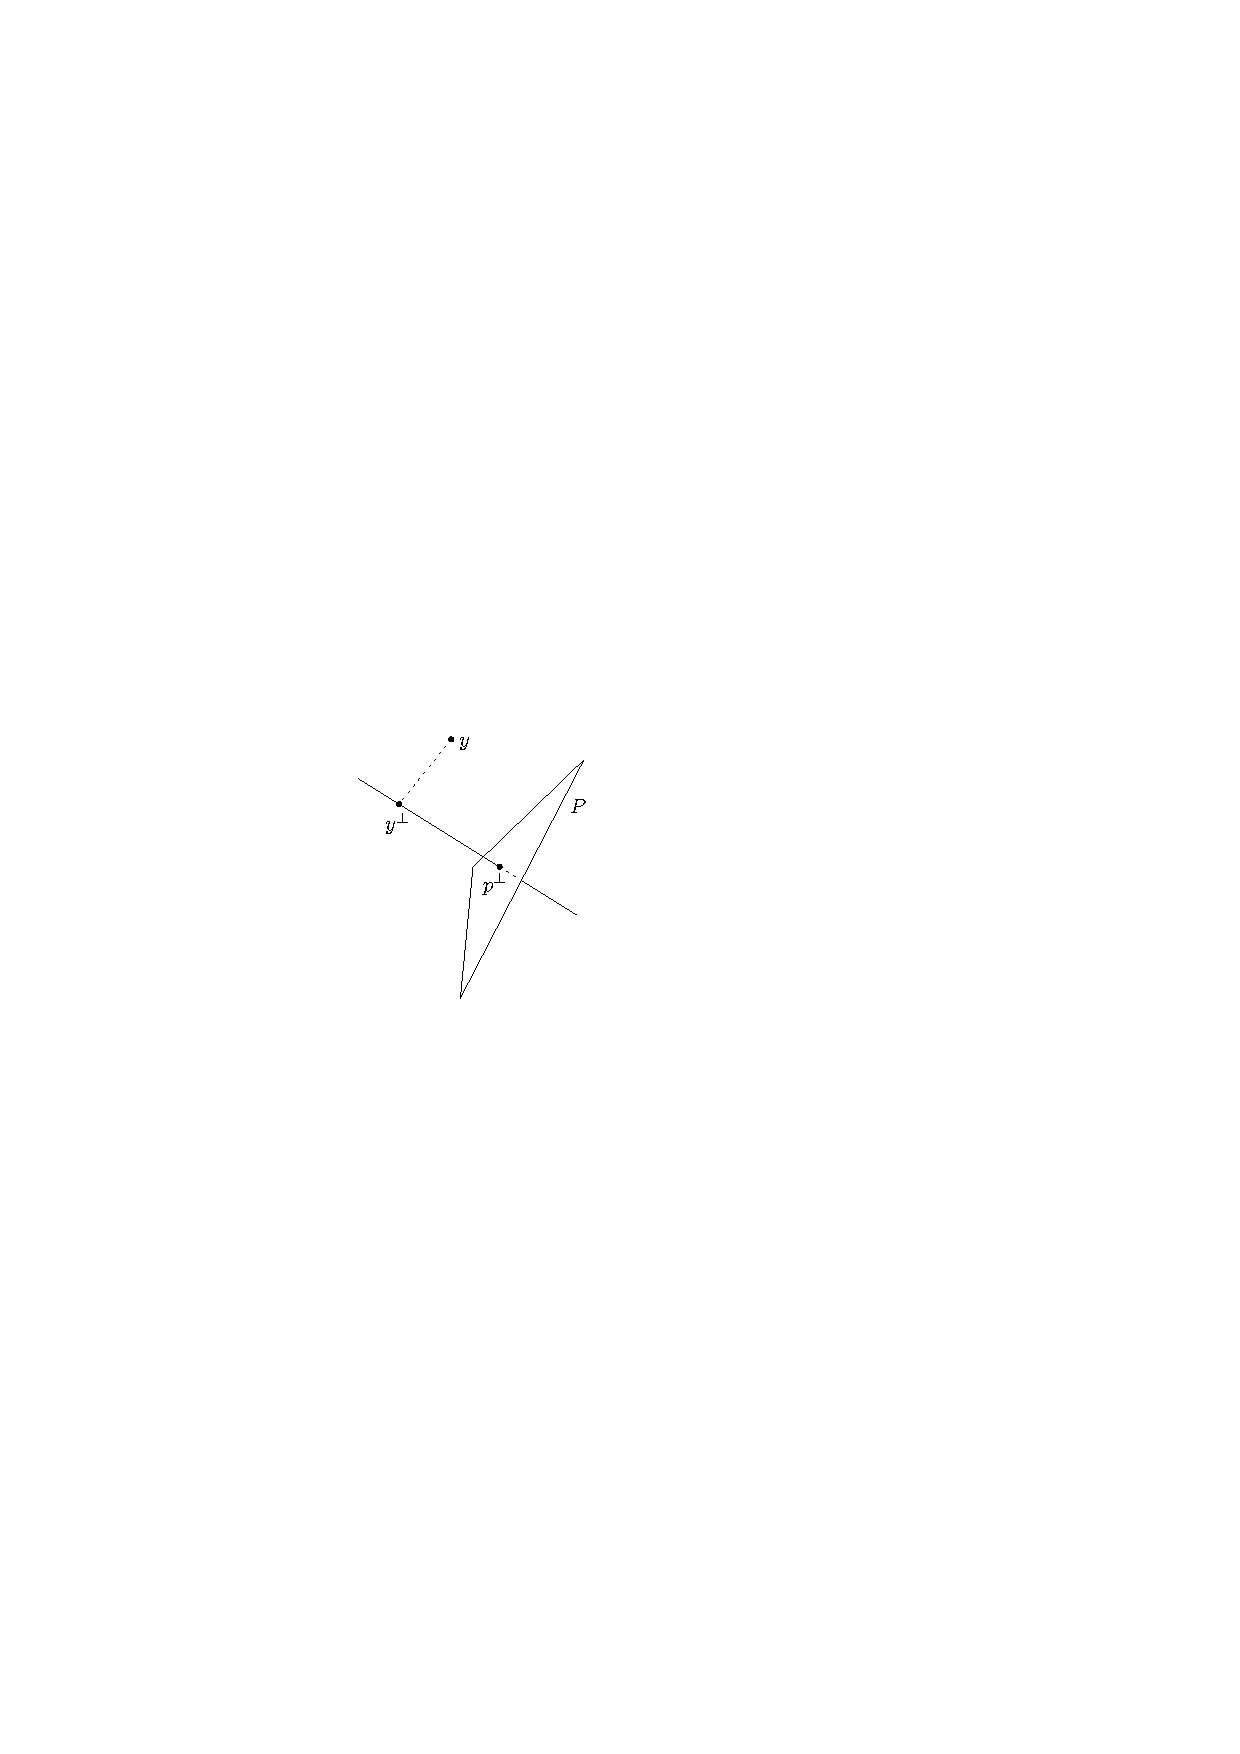
\includegraphics[width=0.26\textwidth]{pics/projection.pdf}
  \end{center}
  \caption{The projection of $y$ and $P$}
  \label{fig:projection}
\end{figure}
We denote by $y^{\perp}$ the projection of a point $y$ on a line perpendicular to the $d-1$ dimensional simplex $P$ (see Figure~\ref{fig:projection}), and by $\|pq\|$ the Euclidean distance between points $p$ and $q$. Let $p$ be any point on $P$, then
\renewcommand{\frac}[2]{(#1/#2)}
    \[  
  \begin{aligned} 
    \vol(c_{i+1},P)-\vol(c_i,P)|
    & =  \frac{1}{d}  \vol_{d-1}(P) \; \left|\; \|c_i^{\perp}p^{\perp}\| -\|c_{i+1}^{\perp} p^{\perp}\|\;\right| \\
    &    \leq \frac{1}{d}  \vol_{d-1}(P)   \|c_i^{\perp}c_{i+1}^{\perp}\|\\
     &  \leq \frac{1}{d} \vol_{d-1}(P) \|\frac{1}{n}x^{\perp} p_{i+1}^{\perp}\|  \enspace .\\
  \end{aligned}
    \]
Then if $x^\perp$ and $p_{i+1}^{\perp}$ are on the same side of the hyperplane
supporting $P$, we have
\[  
  \begin{aligned}
   \frac{1}{d} \vol_{d-1}(P) \|\frac{1}{n}x^{\perp} p_{i+1}^{\perp}\| 
     &  \leq \frac{1}{nd} \vol_{d-1}(P) 
                     \;\left|\;\|x^{\perp}p^{\perp}\|-\|p_{i+1}^{\perp} p^{\perp}\|\;\right| \\
      & \leq\frac{1}{n} |\vol(p_{i+1},P)-\vol(x,P)|\\
  & \leq \frac{1}{n}\sum_{Q \in \binom{P}{d-1}} \vol(x,p_{i+1}, Q) 
  \end{aligned}
\]
Otherwise if $x^\perp$ and $p_{i+1}^{\perp}$ are on different
sides of the hyperplane supporting $P$, we have $\|x^{\perp}
p_{i+1}^{\perp}\|=\|x^{\perp}p^{\perp}\| +\|p_{i+1}^{\perp} p^{\perp}\|$.
In this case the two simplices $Px$ and $Pp_{i+1}$ are disjoints and
the convex hull of $Pxp_{i+1}$ is covered by the union of the simplices
$Qxp_{i+1}$ for $Q \in \binom{P}{d-1}$ (see Figure~\ref{fig:disjSimp}),
\begin{figure}[htb]
  \begin{center}
    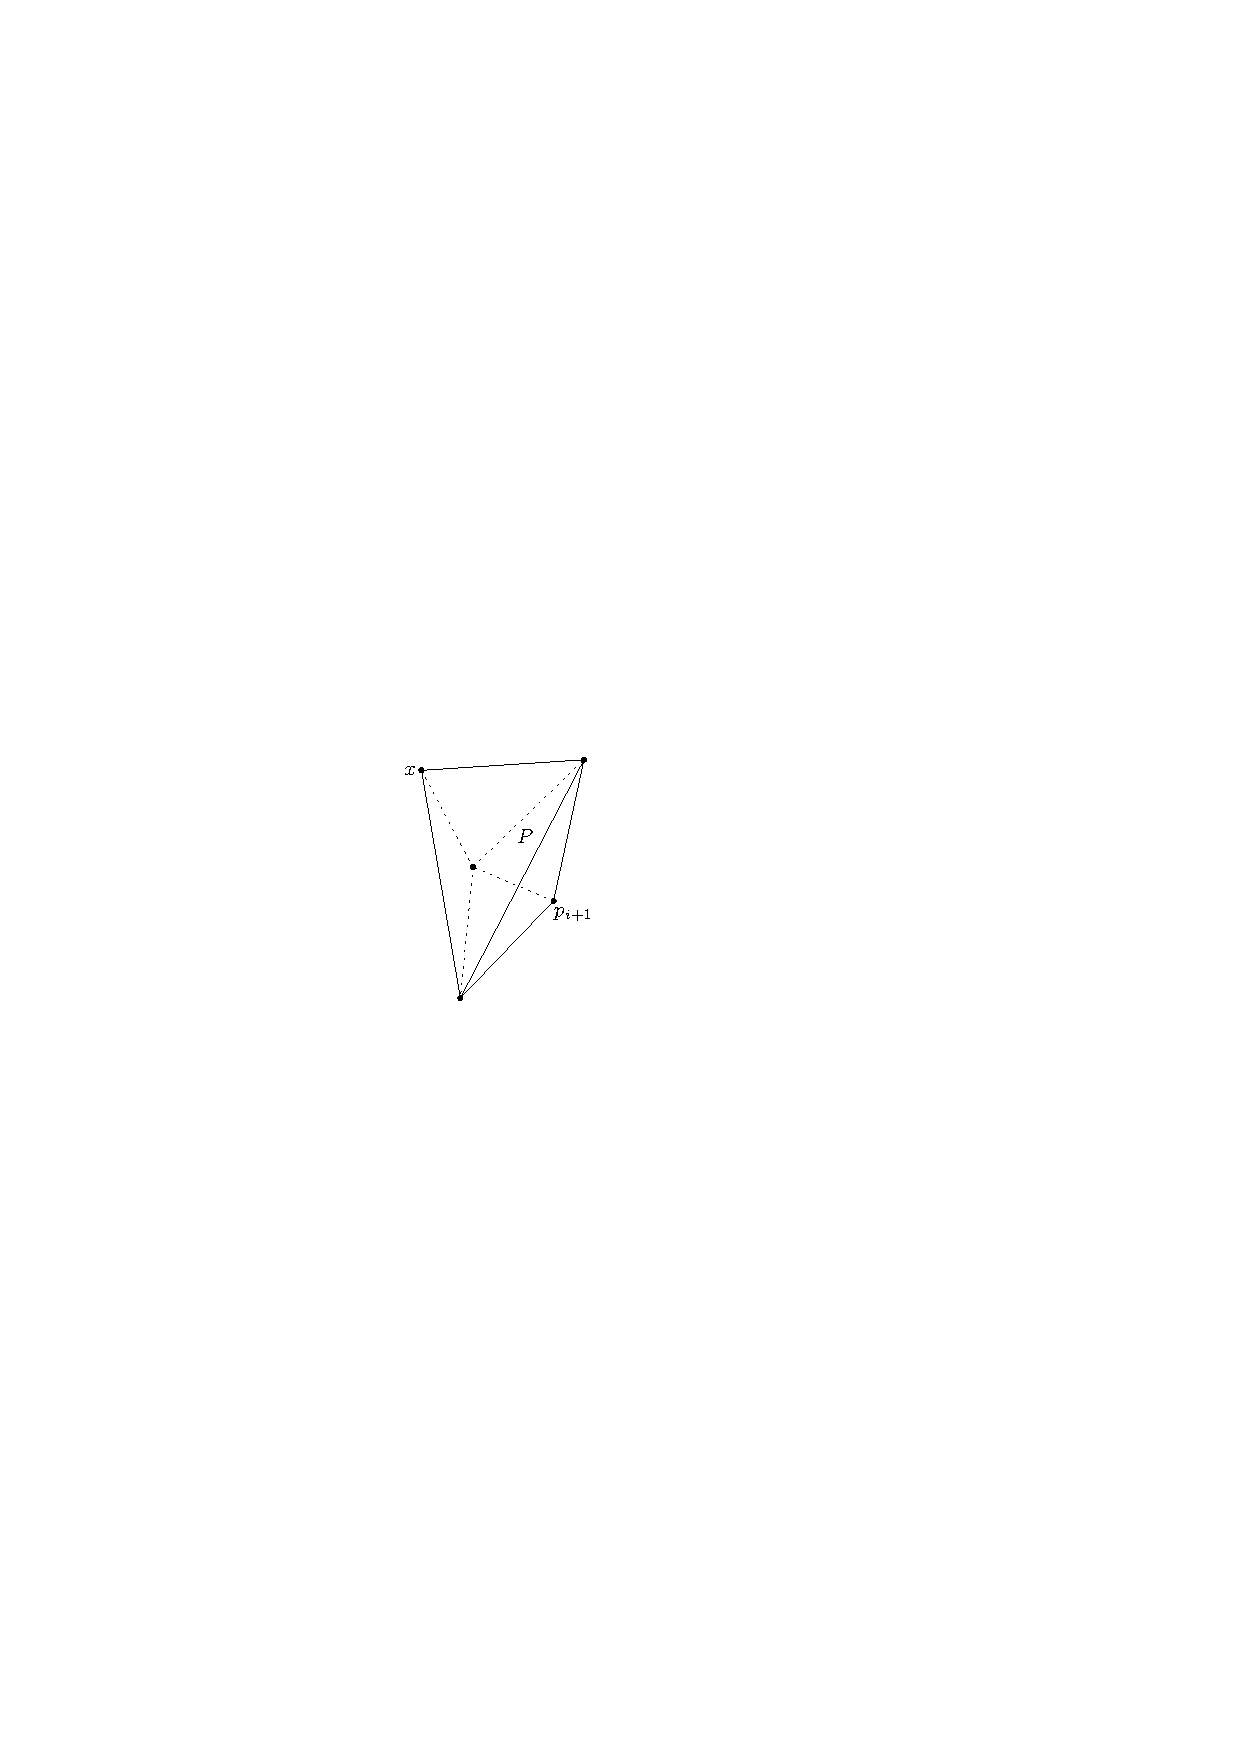
\includegraphics[width=0.22\textwidth]{pics/disjointSimp.pdf}
  \end{center}
  \caption{Point $x$ and $p_{i+1}$ are different sides of $P$}
  \label{fig:disjSimp}
\end{figure}
thus
\[  
  \begin{aligned}
  \frac{1}{d} \vol_{d-1}(P) \|\frac{1}{n}x^{\perp} p_{i+1}^{\perp}\|  
     &  \leq \frac{1}{nd} \vol_{d-1}(P) (\|x^{\perp}p^{\perp}\|+\|p_{i+1}^{\perp} p^{\perp}\|) \\
      & \leq\frac{1}{n} ( \vol(p_{i+1},P)+\vol(x,P) )\\
  & \leq \frac{1}{n}\sum_{Q \in \binom{P}{d-1}} \vol(x,p_{i+1}, Q) 
 \end{aligned}
\]
We can now prove that $(\ref{eq:i})\leq(\ref{eq:o})$ as follows:
\[
  \begin{aligned}
  \sum_{P \in \binom{S_i}{d}} (\vol(c_{i+1}, P)- \vol(c_i,P))
 & \le \sum_{P \in \binom{S_i}{d}} |\vol(c_{i+1}, P)- \vol(c_i,P)| \\
 & \le \frac{1}{n} \sum_{P \in \binom{S_i}{d}} \sum_{K \in \binom{P}{d-1}} \vol(x,p_{i+1}, K) \\
  & \le \frac{(n-(d-1))}{n} \sum_{K \in \binom{S_i}{d-1}}  \vol(x,p_{i+1}, K) \enspace .
  \end{aligned}
\]


Next, we show that $(\ref{eq:ii}) \le d\times (\ref{eq:o})$. Applying (\ref{eq:cover}),
\[
  \begin{aligned}
     & \!\!\! \sum_{Q\in \binom{S'}{d-1}}
           (\vol(c_{i+1},p_{i+1},Q)- \vol(c_{i+1},x,Q)) \\
     &\le  \sum_{Q\in \binom{S'}{d-1}} 
           \left(\vol(x,p_{i+1},Q) + \sum_{R \in \binom{Q}{d-2}} \vol(x,p_{i+1},c_{i+1},R)\right) \\
     &\le  \sum_{Q \in \binom{S_i}{d-1}}  \vol(x,p_{i+1}, Q) + (n-1 - (d-2)) \sum_{R \in \binom{S_i}{d-2}} \vol(x,p_{i+1},c_{i+1},R) \enspace .
  \end{aligned}
\]
Let $\svol(p_1, \ldots, p_{d+1})$ denote the signed volume of the simplex with vertices $p_1, \ldots, p_{d+1}$. By linearity of the determinant we have
\[
  \begin{aligned}
    \svol(x,p_{i+1},c_{i+1},R) & = \frac{1}{n} \sum_{y \in S_{i+1}} \svol(x,p_{i+1},y,R) \\
  & = \frac{1}{n} \sum_{y \in S_{i}} \svol(x,p_{i+1},y,R)
  \end{aligned}
\]
Since the absolute value of the sum can be bounded by the sum of the absolute values, we get
\[
\vol(x,p_{i+1},c_{i+1},R) \le \frac{1}{n} \sum_{y \in S_{i}} \vol(x,p_{i+1},y,R),
\]
and thus
\[
\sum_{R \in \binom{S_i}{d-2}} \vol(x,p_{i+1},c_{i+1},R) \leq \frac{(d-1)}{n}\sum_{Q \in \binom{S_i}{d-1}}  \vol(x,p_{i+1}, Q).
\]
Thus we can get $(\ref{eq:ii}) \le d\times (\ref{eq:o})$.


Finally, we resubstitute to obtain
\[
  \begin{aligned}
     \od(c_{i+1},S_{i+1})
     &\le \od(c_{i},S_{i}) + (d+1) \sum_{Q\in\binom{S_i}{d-1}} \vol(x,p_{i+1},Q)\\
     &\le (d+1) \od(x,S_{i}) + (d+1) \sum_{Q\in\binom{S_i}{d-1}} \vol(x,p_{i+1},Q) \\
     & = (d+1) \od(x,S_{i+1})  \enspace .
  \end{aligned}
\]
Thus we have $\od(\cog(S),S) \le (d+1)\od(x,S)$, completing the proof.
\end{proof}

We remark that Lemma~\ref{lem:grav1d} and Theorem~\ref{thm:gravdd} are essentially the best possible. To see this, take the multiset $S$ that contains $n-d$ copies of the origin $o$, and each of the remaining $d$ points has one different coordinate $1$ and all other coordinates $0$. In this case $\od(o, S)= 1/d!$ and $\od(\cog(S), S)= (d + 1 - O(d^2/n))\times 1/d!$.

\section{Conclusion}
\label{sec:concl}

We have given several results relating Oja depth and centers of mass.
There are several directions for future work.

We do not know of any point set that gives a lower-bound matching the
upper-bound of Theorem~\ref{thm:ndcenter}. The best lower-bound we know
is that placing $n/(d+1)$ points at each vertex of any $d$-simplex of
unit volume yields to an Oja depth of $n^d / (d+1)^{d}$ for any point
inside the simplex.  For $d=2$, for example, Theorem~\ref{thm:ndcenter}
implies $\od(x, S)\le n^2/6 - O(n)$ where as the best lower bound (above)
has $\od(x, S)\ge n^2/9$.  This construction leads us to the following
conjecture:
\begin{conj}
For any point set $S\subset\R^d$ whose convex hull has unit volume, there exists $x\in\R^d$, such that $\od(x,S)\le n^d / (d+1)^{d}$
\end{conj}


\bibliographystyle{abbrv}
\bibliography{ojacenter}

\end{document}
